\documentclass{beamer}
\mode<presentation>
\usetheme{Madrid}
\usepackage{amsfonts,amsmath,amsthm,amssymb}
\usepackage{graphicx,graphics}
\usepackage{setspace,fontspec}
\usepackage[utf8x]{inputenc}
\newcommand*{\utb}{\item[{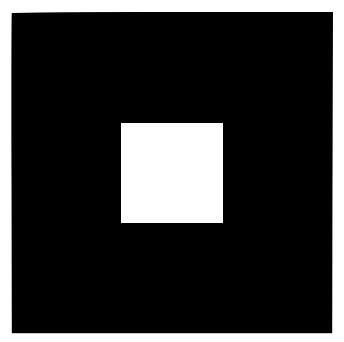
\includegraphics[width=0.3cm]{img/UTSymbols-Bullet.png}}]}
\renewcommand*{\thefootnote}{\fnsymbol{footnote}}
\newcommand{\sign}[1]{\ensuremath{\operatorname{sign(\mathit{#1})}}}

\setsansfont[Path = fonts/, UprightFont=UTSans-Medium.otf, BoldFont=UTSans-Bold.otf]{}

\title{\bf Inteligența artificială}
\author[matei.sirbu@student.unitbv.ro]{Sîrbu Matei-Dan}
\institute[UniTBv]{Universitatea Transilvania din Brașov \\ Facultatea de Matematică și Informatică}
\date{3 decembrie 2020}

\definecolor{albastruMI}{rgb}{0, 0.23, 0.49}
\setbeamercolor*{palette primary}{bg=albastruMI, fg = white}
\setbeamercolor*{palette secondary}{bg=albastruMI, fg = white}
\setbeamercolor*{palette ternary}{bg=albastruMI, fg = white}
\setbeamercolor*{palette quaternary}{bg=albastruMI, fg = white}
\setbeamercolor*{author in head/foot}{parent=palette primary}
\usefonttheme[onlymath]{serif}
\setstretch{1.5}

\begin{document}
\frame{\titlepage}

\begin{frame}
    \frametitle{Inteligența artificială și învățarea automată}
    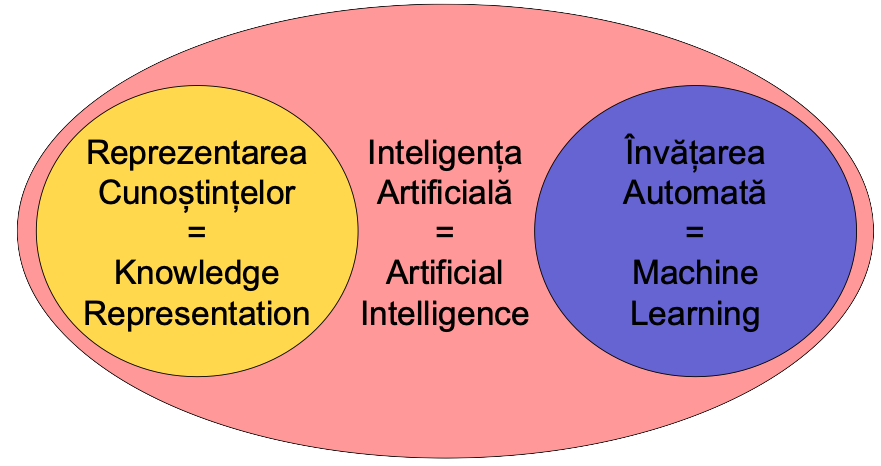
\includegraphics[width=1\textwidth]{img/venn}
\end{frame}

\begin{frame}
    \frametitle{La ce se referă inteligența artificială?}
    \begin{itemize}
        \utb Scopul suprem al inteligenței artificiale este de a construi sisteme care să atingă nivelul de inteligență al omului
        \utb Testul Turing: un computer prezintă un nivel de inteligență uman dacă un interlocutor uman nu reușește să distingă, în urma unei conversații în limbaj natural, că vorbește cu un om sau cu un calculator
    \end{itemize}
    \begin{center}
        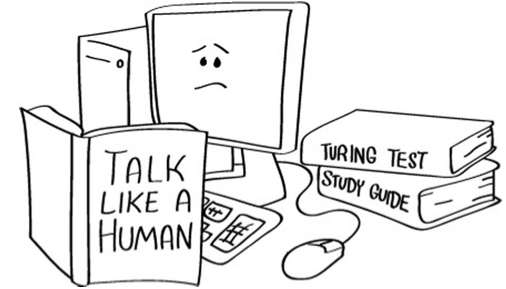
\includegraphics[width=0.4\textwidth]{img/talk_like_a_human}
    \end{center}
\end{frame}

\begin{frame}
    \frametitle{La ce se referă învățarea automată?}
    \begin{itemize}
        \utb O mare parte din cercetători consideră că acest scop poate fi atins prin imitarea modului în care o oamenii învață
        \utb \textbf{Învățarea automată} – domeniu care studiază modul în care calculatoarele pot fi înzestrate cu abilitatea de a învăța, fără ca aceasta să fie programată în mod explicit
        \utb În acest context, \textbf{învățarea} se referă la recunoașterea unor tipare / structuri (patterns) complexe și la luarea deciziilor inteligente bazate pe observațiile din \textbf{date}
    \end{itemize}
\end{frame}

\begin{frame}
    \frametitle{Problemă ,,bine pusă'' de învățare automată}
    \begin{itemize}
        \utb Ce probleme pot fi rezolvate\footnote[frame]{rezolvate cu un anumit grad de acuratețe} folosind învățarea automată?
        \utb \textbf{Problemă ,,bine pusă'' de învățare automată:}
        \utb Spunem despre un program pe calculator că învață dintr-o experiență E în raport cu o clasă de task-uri T și o măsură de performanță P, dacă performanța sa în rezolvarea task-urilor T, măsurată prin P, se îmbunătățește odată cu experiența E
    \end{itemize}
\end{frame}

\begin{frame}
    \frametitle{Problemă ,,bine pusă'' de învățare automată}
    \begin{itemize}
        \utb Arthur Samuel (1959) a scris un program pentru a juca dame (probabil primul program bazat pe conceptul de învățare)
        \utb Programul a jucat împotriva lui însuși 10 mii de jocuri
        \utb Programul a fost conceput să găsească ce poziții ale tablei de joc erau bune sau rele în funcție de probabilitatea de a câștiga sau pierde
    \end{itemize}
    \begin{minipage}[b]{0.5\textwidth}
        \begin{itemize}
            \utb În acest caz:
            \utb E = 10000 de jocuri
            \utb T = joacă dame
            \utb P = dacă câștigă sau nu
        \end{itemize}
    \end{minipage}
    \begin{minipage}[b]{0.4\textwidth}
        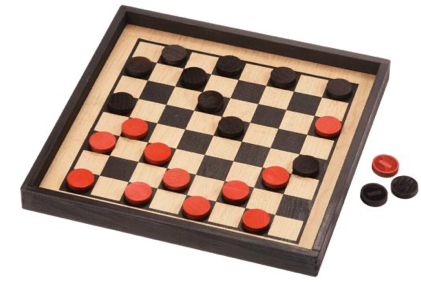
\includegraphics[width=\textwidth]{img/checkers}
    \end{minipage}
\end{frame}

\begin{frame}
    \frametitle{Când se aplică învățarea automată?}
    \begin{itemize}
        \utb Se aplică în situații în care este foarte greu (imposibil) să definim un set de reguli de mână / să scriem un program
        \utb Exemple de probleme unde putem aplica învățarea automată:
        \utb Detectarea facială
        \utb Înțelegerea vorbirii
        \utb Prezicerea prețului acțiunilor
        \utb Recunoașterea obiectelor
    \end{itemize} 
\end{frame}  

\begin{frame}
    \frametitle{Esența învățării automate}
    \begin{itemize}
        \utb Există un tipar
        \utb Dar nu îl putem exprima programatic / matematic
        \utb Avem date / exemple în care regăsim acest tipar
    \end{itemize}
    \begin{center}
    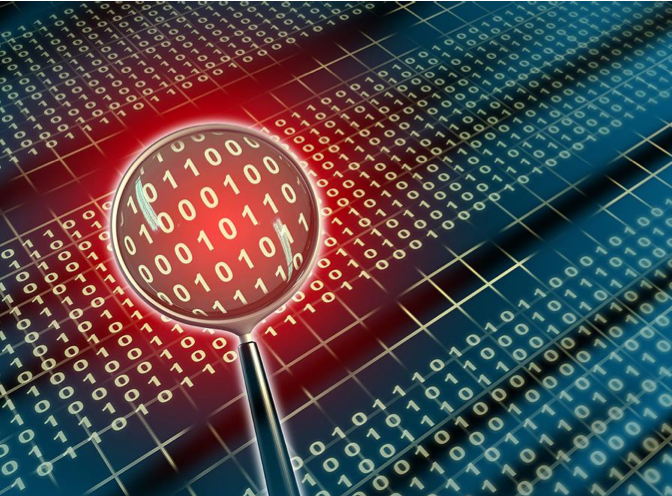
\includegraphics[width=0.49\textwidth, height=4cm]{img/bits_magnifier}
    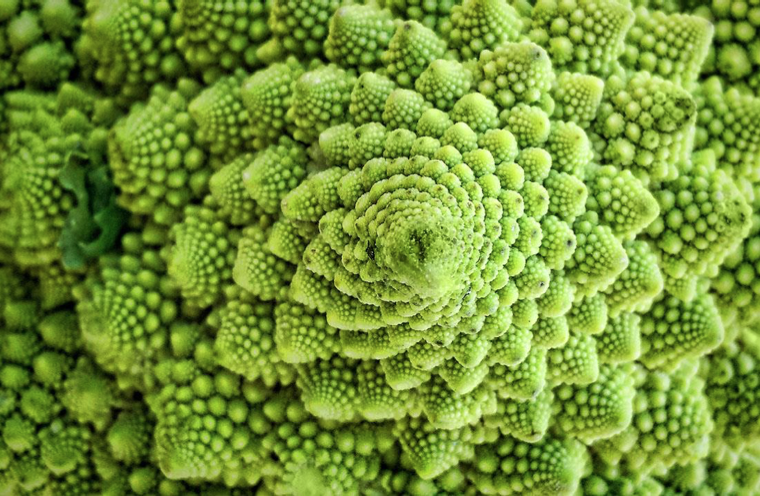
\includegraphics[width=0.49\textwidth, height=4cm]{img/fractal_pattern}
    \end{center}
\end{frame}

\begin{frame}
    \begin{center}
        \huge Programare tradițională
        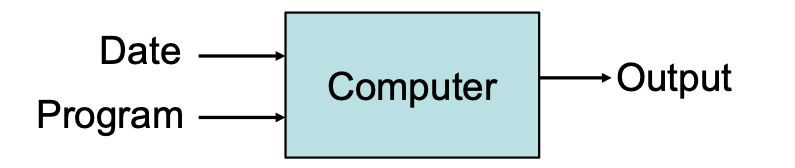
\includegraphics[width=10cm]{img/traditional_learning}
    \end{center}
    \begin{center}
        \huge Învățare automată
        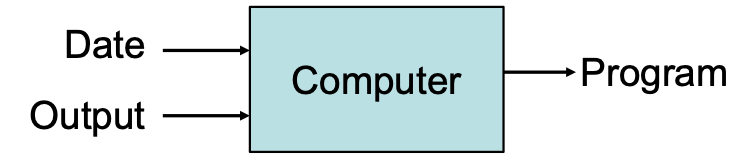
\includegraphics[width=10cm]{img/automated_learning}
    \end{center}
\end{frame}

\begin{frame}
    \frametitle{Scurt istoric al inteligenței artificiale}
    \begin{itemize}
        \utb Anii 1960-1980: ,,AI Winter''
        \utb Anii 1990: Rețelele neuronale domină, în principal datorită descoperirii algoritmului de propagare a erorii înapoi pentru rețele cu mai multe straturi
        \utb Anii 2000: Metodele kernel domină, în principal din cauza instabilității rețelelor neuronale
        \utb Anii 2010: Revenirea la rețele neuronale, în principal datorită conceptului de învățare profundă (deep learning)
    \end{itemize}
\end{frame}

\begin{frame}
    \frametitle{De ce funcționează în prezent?}
    \begin{minipage}[t!]{0.45\textwidth}
        \begin{itemize}
            \utb Mai multă putere de calcul
            \utb Mai multe date
            \utb Modele mai bune
        \end{itemize}
    \end{minipage}
    \begin{minipage}[t!]{0.54\textwidth}
        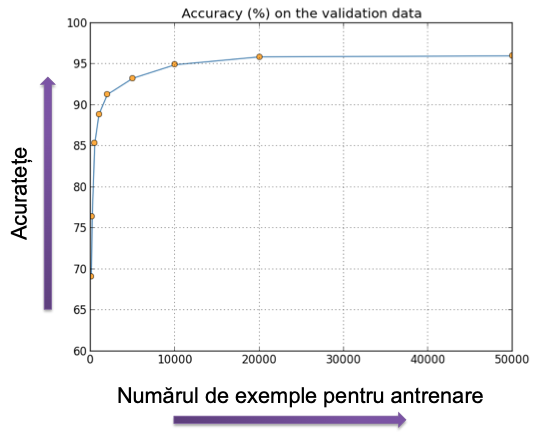
\includegraphics[width=\textwidth]{img/accuracy_on_validation_data}
    \end{minipage}
\end{frame}

\begin{frame}
    \frametitle{Esența învățării automate}
    \begin{itemize}
        \utb Mii de algoritmi de învățare automată existenți
        \begin{itemize}
            \utb Cercetătorii publică sute de noi algoritmi în fiecare an
        \end{itemize}
        \utb Simplificând decenii de cercetare în domeniu, putem
        reduce învățarea automată la:
        \begin{itemize}
            \utb Învățarea unei funcții $f$ care să mapeze un input $X$ către un output $Y$, anume $f:X \rightarrow Y$
            \utb Exemplu: $X:$ email-uri, $Y:\{\text{spam, non-spam}\}$
        \end{itemize}
    \end{itemize}
\end{frame}

\begin{frame}
    \frametitle{Esența învățării automate}
    \begin{itemize}
        \utb Input: $X$ (imagini, texte, email-uri...)
        \utb Output: $Y$ (spam sau non-spam...)
        \utb Funcție target (necunoscută) \\ $f : X \rightarrow Y$ (realitatea / ,,adevărata mapare'')
        \utb Date \\ $(x_1, y_1), (x_2, y_2), \dots (x_N, y_N)$
        \utb Model \\ $g : X \rightarrow Y$ \\ $y = g(x) = \sign{w^Tx}$
    \end{itemize}
\end{frame}

\begin{frame}
    \frametitle{Esența învățării automate}
    \begin{itemize}
        \utb Orice algoritm de învățare automată are 3 componente:
        \begin{itemize}
            \utb Reprezentare / Modelare
            \utb Evaluare / Funcție obiectiv
            \utb Optimizare
        \end{itemize}
    \end{itemize}
\end{frame}

\begin{frame}
    \frametitle{Ce cunoștințe sunt necesare?}
    \begin{center}
        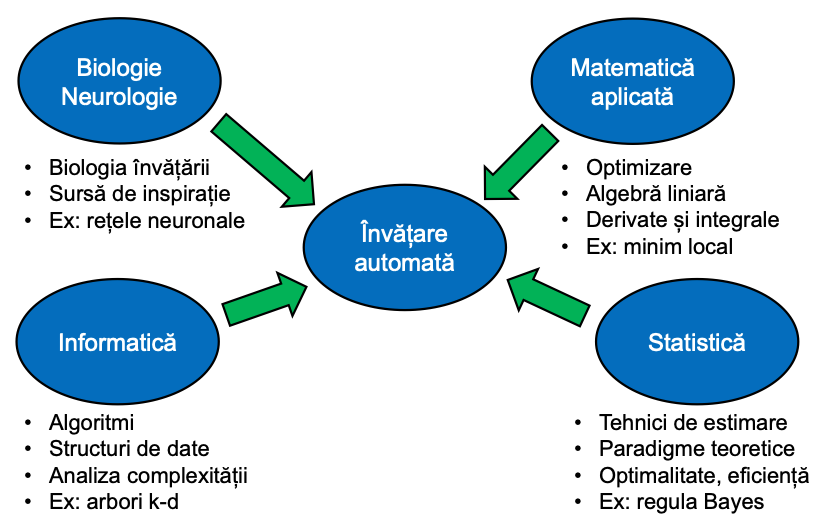
\includegraphics[width=0.9\textwidth]{img/knowledge_required}
    \end{center}
\end{frame}

\end{document}